\documentclass{article}



\usepackage{arxiv}

\usepackage[utf8]{inputenc} % allow utf-8 input
\usepackage{fontspec}
\usepackage[slantfont, boldfont]{xeCJK}

\usepackage[T1]{fontenc}    % use 8-bit T1 fonts
\usepackage{hyperref}       % hyperlinks
\usepackage{url}            % simple URL typesetting
\usepackage{booktabs}       % professional-quality tables
\usepackage{amsfonts}       % blackboard math symbols
\usepackage{nicefrac}       % compact symbols for 1/2, etc.
\usepackage{microtype}      % microtypography
\usepackage{lipsum}		% Can be removed after putting your text content
\usepackage{graphicx}
\usepackage{natbib}
\usepackage{doi}
\usepackage{amsmath, amsthm, amssymb, bm, graphicx, mathrsfs}
\usepackage{graphicx}
\usepackage{subfigure}
% \counterwithin{figure}{section}

\title{A graph-based solver in the university course timetable scheduling\\
一个基于图着色的大学课程排课求解器}
% \date{September 9, 1985}	% Here you can change the date presented in the paper title
%\date{} 					% Or removing it

% \author{Chongfeng Ling\\1716474}

\author{ \hspace{1mm}Chongfeng Ling \\
	1716474\\
	Department of Applied Mathematics\\
	Xi'an Jiaotong-Liverpool University\\
	\texttt{Chongfeng.Ling17@student.xjtlu.edu.cn} \\
	%% examples of more authors
	\And
	% \href{https://orcid.org/0000-0000-0000-0000}{
\includegraphics[scale=0.06]{orcid.pdf}\hspace{1mm}Elias D.~Striatum} \\
	% Department of Electrical Engineering\\
	% Mount-Sheikh University\\
	% Santa Narimana, Levand \\
	% \texttt{stariate@ee.mount-sheikh.edu} \\
	% \AND
	M.B.N. (Thijs) Kouwenhoven \\
	Supervisor \\
	Head, Department of Physics \\
	Xi'an Jiaotong-Liverpool University\\
	\texttt{t.kouwenhoven@xjtlu.edu.cn} \\
	% \And
	% Coauthor \\
	% Affiliation \\
	% Address \\
	% \texttt{email} \\
	% \And
	% Coauthor \\
	% Affiliation \\
	% Address \\
	% \texttt{email} \\
}

% Uncomment to remove the date
% \date{December 1, 2021}

% Uncomment to override  the `A preprint' in the header
\renewcommand{\headeright}{Interim Report}
\renewcommand{\undertitle}{Interim Report}
\renewcommand{\shorttitle}{Timatable Problem}

%%% Add PDF metadata to help others organize their library
%%% Once the PDF is generated, you can check the metadata with
%%% $ pdfinfo template.pdf
% \hypersetup{
% pdftitle={A template for the arxiv style},
% pdfsubject={q-bio.NC, q-bio.QM},
% pdfauthor={David S.~Hippocampus, Elias D.~Striatum},
% pdfkeywords={First keyword, Second keyword, More},
% }

\begin{document}
\maketitle

% \begin{abstract}
% 	% \lipsum[1]
% 	\begin{center}
% 		None
% 	\end{center}
% \end{abstract}

% keywords can be removed
% \keywords{Timetable Scheduling \and Graph Coloring \and Tabu Search \and Reinforcement Learning}

\newpage
\tableofcontents
\newpage

\begin{abstract}
	% \begin{center}
	Timetabling problem is popular in various areas and can be formulated to graph coloring problem. We consider a simple kind - the university timetabling problem in XJTLU as our target problem. Due to the large scale number of people and constrains, we use and modify a heuristic algorithm as our solver to built up a timetable system. With the development of Neural Networks and its successful applications in other combinatorial problems, we also attempt to apply Reinforcement Learning to enhance our solver. 
	% \end{center}
\end{abstract}
\keywords{Timetable Scheduling \and Graph Coloring \and Heuristic Algorithm \and Tabu Search \and Reinforcement Learning}

\newpage

\section{Introduction}

Timetable scheduling is a practical problem with applications in several areas including transportation, hospital and education. Every semester one university is supposed to develop timetables for teach activities and examination to meeting students and staffs' requirements and school hardware source limitation. Credit to pervious works, university timetabling has been divide into two interrelated subproblem: timetabling subproblem and grouping subproblem based on graph coloring\citep{(hertz1991)tabu}. While a lot of studies has been spent on this topic, there is still a big gap between algorithm result and practical timetable \citep{(mccollum2006)perspective} mainly due to various constraints of different university and large scale of data. Consider these constraints with a large volume of data, timetable scheduling is a NP-hard or NP-complete problem \citep{(even1975)complexity}, which means it can not be solved in a polynomial time with large scale problem data. Up to now most of solver is based on heuristic algorithm and its variants like meta-heuristic and hyper-heuristic. This paper attempts to implement some heuristic algorithm while introducing a new method Reinforcement Learning to built a system to solve course timetabling problem in Xi'an Jiaotong-Liverpool University (XJTLU).

The structure of this paper is organized as follow. Section \ref{sec: Literature Review} is a review of the development of timetable scheduling including algorithms, computer system and benchmarks. Section \ref{sec: Problem Description} is a problem description based on graph theory. In section \ref{sec: Research Approach} we present methodologies including Tabu Search algorithm and one improved version called TABCOL. Specific execution plan with timeline and challenges is stated in Section \ref{sec: Execution Plan}.

\newpage

\section{Literature Review}
\label{sec: Literature Review}

Since the 1980s, the connection between timetabling problem and graph coloring with heuristic algorithms has been established. In 1985, \citet{(werra1985)introduction} stated a formal way to model course-teacher timetabling and provided formulations in both graph edge coloring and graph node coloring. Then \cite{(hertz1987)using} solved a large scale random graph coloring problem by tabu algorithm and the TABUCOL procedure that reduces number color from maximum value, compared with annealing algorithm, the CPU-time was much shorter and furthermore, for some unsolved graph, tabu algorithm could indicate the "bad" edges that needed to be reduced. The principles and illustrations of Tabu Algorithm were given by \cite{(werra1989)tabu} and later \cite{(glover1990)tabu} mentioned that the advantage of Tabu Search compared other meta-heuristic algorithm owing to its long-term memory. \cite{(hertz1991)tabu} and \cite{(tuga2007)hybrid} used Tabu Algorithm to solved timetabling problem and due to hard constraints can not guarantee the existence of a feasible solution, they first defined the feasible solution respect to soft constraints and optimized it by hard constraints. In addition, \cite{(costa1994)tabu} made a detailed description about timetable problem and mathematical formulation. Based on the property of meta-heuristic, he generated a general Tabu Algorithm which can be adapted under various constraints and used in different university and colleges. In 1997, \cite{(werra1997)combinatorics} added a new constraint to spread lectures uniformly across a set of periods and proved some existence of solutions under some typical constraints. \cite{(schaerf1999)survey} made a survey about how heuristic algorithm could assign timetable automatically. To reduce the influence of parameter choice, a hyper-heuristic algorithm based on Tabu Algorithm was used to solved examination by \cite{(hussin2005)tabu} and \cite{(kendall2005)investigation} which is parameter free. \cite{(galinier2006)survey} modified TABCOL algorithm and made a comparison between four graph coloring method with different search space and search strategies. While an initial feasible solution is needed for all heuristic algorithm, \cite{(burke2007)graphbased} create heuristic algorithm based on graph degree and operate algorithm in a hyper-heuristic search space reduce the difficult of finding a feasible initial solution.

With the development of Neural Network, \cite{(fazelzarandi2020)state} stated the advantages and disadvantages of some neural network algorithm and Tabu Search employed in scheduling. While Attention Mechanism successfully employed in some NLP models with transformer framework \citep{(ashishvaswani2017)attention,(devlin2019)bert}, \cite{(kool2019)attention} had used Attention Mechanism with Reinforcement Learning to solve TSP problem with up to 100 nodes.

There are also some appreciated framework of timetabling systems. \cite{(carter2000)comprehensive} described a comprehensive university timetable system in Waterloo including system structure and algorithm phase. Additionally, he introduced decomposition in both student section and timetable which will reduce algorithm complexity and conflicts. In general, practical problems are more complexity than algorithm theory. \cite{(mccollum2006)perspective} gave a overview on gaps of timetabling problem between theory and practice and bridged the gaps between the two.  \cite{(kristiansen2013)comprehensive} and \cite{(johnes2015)operational} made a review of timetabling scheduling and student section. In addition, \cite{(kristiansen2013)comprehensive} stated most of previous practical research in timetable were founded that they were based on simulation dataset. Hence, they introduced a open-source dataset in Denmark university and its format description. ALTUMA \citep{(tesfaldet2008)automated} was the solver in the University of Asmara which using memetic algorithm, its performance was experienced and evaluated by read data in the university successfully. Moreover, UniTime \citep{(muller2016)reallife} was an open-source system and successfully implemented in a large scale university.


\newpage

\section{Problem Description}
\label{sec: Problem Description}

In this section, we follow the terminology and problem descriptions by \cite{(werra1985)introduction}. According to the \cite{(wren1996)scheduling}, timetabling problem is defined as the allocation to arrange resources into space and time subjects to constrains such that satisfies a set of desirable objectives as many as possible. We will firstly definite sources in university and then list constraints under XJTLU requirement. In gegeral, one curriculum contains several courses while each course could be repeated more than once and thus split into multiple sections. The subproblem of finding the best grouping of students into corresponding course section is called grouping problem. Normally in every week several lectures with corresponding teachers are hold respect to the course. The comprehensive definitions of resources that involved in XJTLU are listed as follow:

\begin{itemize}
	\item Teacher set $T=\left\{t_{1}, \ldots, t_{j}\right\}$
	\item Class set $C=\left(c_{1}, \ldots, c_{i}\right\}$. A class is a group of students who have the same curriculum.
	\item Classroom set $CR=\{cr_{1},...,cr_{ncr}\}$
	\item Requirement matrix $R=(r_{ij})$ gives the number of lectures involving $c_i$ and $t_j$ during one week or day.
	\item A period is a day corresponding to weekly scheduling and each timeslot is a period in daily scheduling.
	\item Course set $CO=\left\{co_{1}, ... , co_{nco}\right\}$. A course is defined by
	      \begin{enumerate}
		      \item a set of teachers
		      \item a set of classes
		      \item a set of lectures $L=\left\{\ell_{1}, \ldots, \ell_{n l}\right\}$
		      \item a set of course sections.
	      \end{enumerate}
\end{itemize}
Based on the above definitions of sources, constraints of the timetable problem are as follow:
\begin{enumerate}
	\item teacher overlaps: a teacher cannot be involved simultaneously in more than one lecture.
	\item class overlaps: a class cannot be involved simultaneously in more than one lecture.
	\item classroom overlaps: a classroom cannot be involved simultaneously in more than one lecture.
	\item period constraints: the duration of lectures could be one or two hours.
	\item pre-assignment constraints: the lectures are preassigned to a set of specific periods or classrooms.
	\item teacher unavailability: a lecture involving a teacher $t_{j}$ cannot be scheduled at a period during which $t_{j}$ is not available, including lunch break and university free afternoon (i.e. Wednesday afternoon in XJTLU)
	\item  geographical constraints: Two lectures given in two distant classroom should be scheduled consecutively if and only if there is sufficient time for moving one classroom to another.
	\item  compactness constraints: each teacher and student wants a schedule with a minimal number of holes and isolated lectures.
	\item  distribution constraints: the identical lectures (i.e. the lectures of a same course) should be spread as uniformly as possible in weekly scheduling.
\end{enumerate}
Depend on university management, these constraints should be spilt into two parts: one is hard constraints and the other is soft constraints. While optimizing, a feasible solution is the one which satisfied all hard constraints, moreover, the optimal one is a feasible solution and satisfies all soft constraints.


\subsection{Mathematical formulation: A Graph Coloring representation}

Consider a basic course scheduling model in daily scheduling. For one course $co_a$ with a set of lectures $L=\left\{\ell_{1}, \ldots, \ell_{nl}\right\}$, we denote a lecture-node $m_{ab}$ for each course $co_a$ and lecture $l_b$. Due to the class overlaps constraint, all pairs of lecture note in course $co_a$ are connected by edges. While assume all courses have no sections, if there is a student taking both courses $co_{a1}$ and $co_{a2}$, we introduce an edge between every pair of lecture node $m_{a1b}$ and $m_{a2b}$. The feasible course scheduling among $p$ periods is respect to the node coloring of graph G with $p$ colors. An example is given in Figure \ref{Fig.main}. Here we have 3 courses and each of them has 1, 2 or 3 lectures. Student group A takes courses $co_1$ and $co_2$, another group B takes $co_2$ and $co_3$. A feasible solution is drawn by 5 colors, which means at least 5 periods is needed to assign courses without conflicts.

With pre-assignment constraints and teacher unavailability, we introduce two constraints samples: 1. $co_{1}$ not scheduled at period 1; 2. one lectures of $K_{3}$ at period 1 or 3. A set of period nodes are added to Figure \ref{Fig.sub.1} and then we get Figure \ref{Fig.sub.2}. Easy to see that pre-assignment of periods are equal to teacher time unavailability.

\begin{figure}[htbp]
	\centering  %图片全局居中
	\subfigure[without constrain ]{
		\label{Fig.sub.1}
		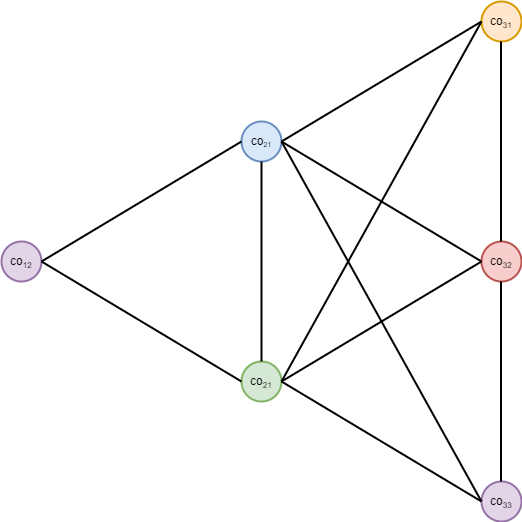
\includegraphics[width=0.45\textwidth]{fig1}}
	\subfigure[with constraints]{
		\label{Fig.sub.2}
		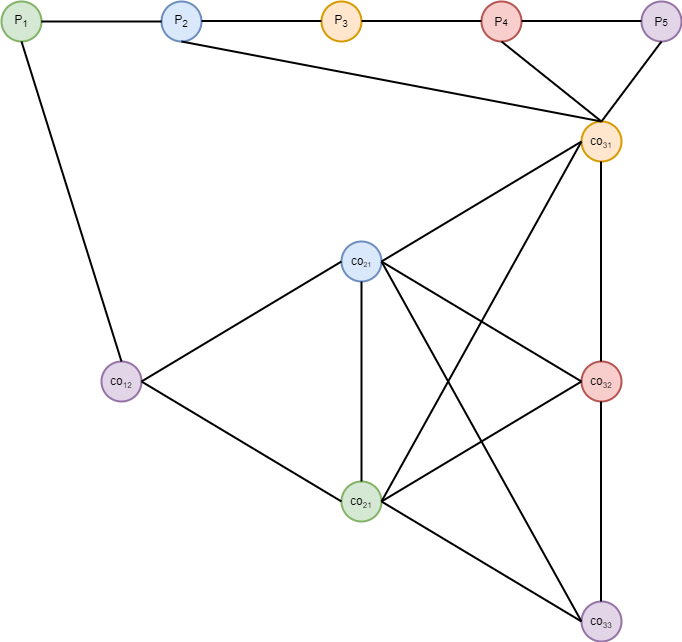
\includegraphics[width=0.45\textwidth]{fig2}}
	\caption{Graph Coloring representation}
	\label{Fig.main}
\end{figure}

\newpage

\section{Research Approach}
\label{sec: Research Approach}

\subsection{Methodology}

\subsubsection{Tabu Search}

Tabu Search is a heuristic algorithm designed for finding a global optimal point and has been used for solving combinatorial optimization problem including graph node coloring, large scale timetabling and TSP efficiently. The basic process is given a feasible solution as initial point and an aspiration function to evaluate results, moving the initial point to another solution in the neighbor of the initial point and making comparison and recording the better solution by aspiration function. The algorithm does not stop until get a global optimum or reach the max number of iterations. The core of Tabu Search algorithm is tabu list $T$ that all moves back to current point are forbidden in the next $|T|$ iterations. TABCOL\citep{(hertz1987)using} is a modified version of Tabu search for coloring of graph. It first initializes a random solution with a large enough number $k$, then use Tabu to reduce the conflicts of edges and obtain a feasible $k$-color graph as an initialization solution for next iteration until get a smallest color set for the graph.

% \begin{figure}
% 	\centering
% 	\includegraphics[width=0.7textwidth]{图片文件名称}
% 	\caption{图片标题名称}label{fig1}
% 	\end{figure}

\begin{figure}[h]
	\centering
	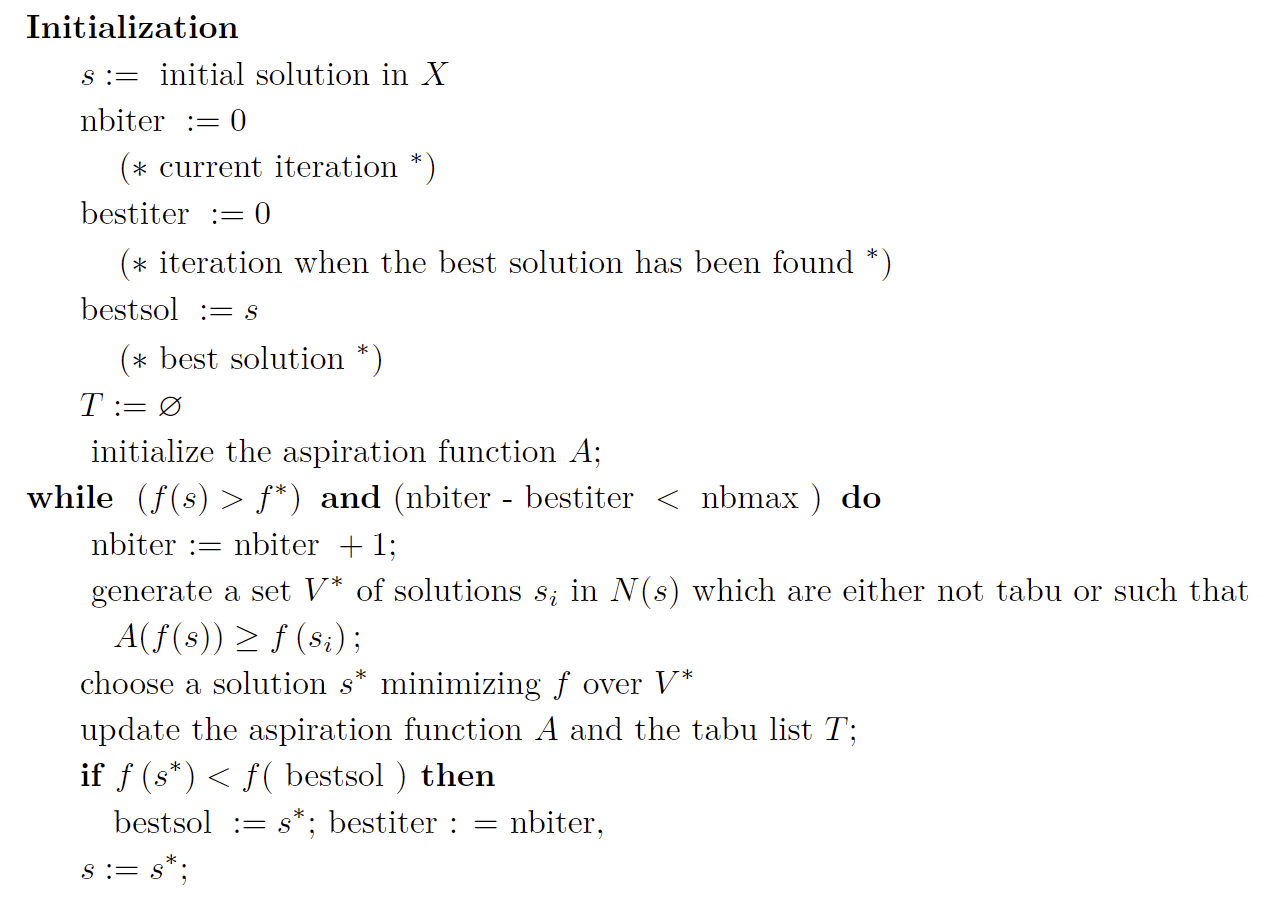
\includegraphics[width=0.8\linewidth]{fig3.png}
	\caption{General Tabu Search Algorithm \citep{(hertz1991)tabu}}
\end{figure}

\subsection{Data collection}

There are two ways to collect data. The first is using open-source datasets in UniTime and also the corresponding benchmarks. To deal the real problem in XJTLU, we first collect high level students in applied mathematics, then consider course sections, data of students with fundamental mathematics couse is the third benchmark for our system. 

\newpage

\section{Execution Plan}
\label{sec: Execution Plan}
\subsection{Timeline}
\begin{itemize}
	\item Programming system
	      \begin{enumerate}
		      \item Data collection. Timeline: before the winter holidays.
		            \begin{enumerate}
			            \item Collect and save online data in University Course Timetabling Data Format (v2.4) \footnote{\url{https://www.unitime.org/uct_dataformat_v24.php}}, write and save data in Python.
			            \item Consider the course section and complexity of problems, we collect real data in XJTLU, 2021-2022 academic year, as follow:
			                  \begin{enumerate}
				                  \item Year 4 applied mathematics students
				                  \item Year 4 applied mathematics and finical mathematics students
				                  \item Year 1 students with fundamental mathematics course.
			                  \end{enumerate}
		            \end{enumerate}
	      \end{enumerate}
	\item Algorithm
	      \begin{enumerate}
		      \item Tabu Algorithm improvement
		            \begin{enumerate}
						\item general TABCOL implemented in timetabling subproblem and grouping subproblem. Timeline: Dec. 1 - Dec. 10.
						\item use matrix to speed up Tabu Search. Timeline: Dec. 10 - Dec. 20.
						\item try hybrid method to find the feasible initial solution for Tabu search automatically. Timeline: Dec. 20 - Jun. 10.
						\item use graph decomposition algorithm to reduce edges in the graph. Timeline: Jun. 10 - Jun. 25.
		            \end{enumerate}
		      \item Attention Mechanism and Reinforcement Learning
		            \begin{enumerate}
			            \item Attention Mechanism. Timeline: Jun. 25 - Feb. 5
			            \item Reinforcement Learning. Timeline: Feb. 5 - Feb. 20
			            \item Attention Mechanism with RL in TSP. Timeline: Feb. 20 - Feb. 28
			            \item real timetable scheduling problem in XJTLU. Timeline: semester 2.
		            \end{enumerate}
	      \end{enumerate}
\end{itemize}

\subsection{Skills and Knowledge}
\begin{enumerate}
	\item \textbf{Graph theory}: learn how to color a graph and the method to reduce edge and decomposition of a big graph.
	\item \textbf{Tabu Search}: learn its idea and variants in graph coloring and scheduling area.
	\item \textbf{Reinforcement Learning}: it is a fast developed Neural Network and more applications appears in combinatorial operational problems. Study its principle and usage in scheduling problem.
	\item \textbf{Plotting graph in Python}: there are many packages to plot in python, learn one of them to obtain visual, or even interactive graphs to help understand.
\end{enumerate}

\subsection{Challenges}
\begin{enumerate}
	\item \textbf{Lack of computing resources}: Heuristic algorithm is an efficient way to solver graph coloring problem and scheduling problems, due to the complexity of this class of NP-hard problems, however, as nodes of the graph increasing, using Tabu Search to get a result is also time-consuming. Taking TABCOL algorithm for coloring of graph \footnote{\url{https://github.com/pchervi/Graph-Coloring}} as an example, we create a series of graph which the probability of one edge in two random vertices is 0.5 and run it on two-core CPU machine. Figure \ref{fig4} tells that with the increasing of vertices, running time grows exponentially.
	
	\begin{figure}[htbp]
		\centering
		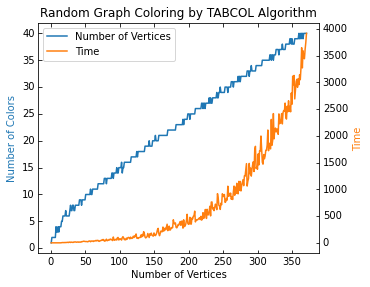
\includegraphics[width=0.6\linewidth]{fig4.png}
		\caption{Random Graph Coloring by TABCOL Algorithm}\label{fig4}
	\end{figure}
	\item \textbf{Deployment of RL algorithm}: Though RL algorithm has been developed in various areas for years, its applications in scheduling problems are rare. Luckily, we can learn another TSP to copy the experiences of how to use Reinforcement Learning algorithm in combinatorial problems, but still there is a long way to applied RL in our project and the difficulty can not be ignored.
\end{enumerate}
\newpage
\qquad

\newpage

\bibliographystyle{agsm}
\bibliography{references}


\end{document}
